\documentclass{beamer}
%\setbeamertemplate{caption}[numbered]{\hfill\inserttitle\hfill}
%\mode<presentation> {


% The Beamer class comes with a number of default slide themes
% which change the colors and layouts of slides. Below this is a list
% of all the themes, uncomment each in turn to see what they look like.

%\usetheme{default}
%\usetheme{AnnArbor}
\usetheme{Antibes}	%good
%\usetheme{Bergen}
%\usetheme{Berkeley}
%\usetheme{Berlin}
%\usetheme{Boadilla}	%theekthak
%\usetheme{CambridgeUS}	%Laal
%\usetheme{Copenhagen}	%theekthak
%\usetheme{Darmstadt}	%jhakaas
%\usetheme{Dresden}
%\usetheme{Frankfurt}
%\usetheme{Goettingen}	%theekthak
%\usetheme{Hannover}
%\usetheme{Ilmenau}
%\usetheme{JuanLesPins}	%Jhakaas
%\usetheme{Luebeck}
%\usetheme{Madrid}	%short titles only
%\usetheme{Malmoe}
%\usetheme{Marburg}	%jhakaas
%\usetheme{Montpellier}	%super se bhi upar
%\usetheme{PaloAlto}
%\usetheme{Pittsburgh}
%\usetheme{Rochester}
%\usetheme{Singapore}
%\usetheme{Szeged}
%\usetheme{Warsaw}

% As well as themes, the Beamer class has a number of color themes
% for any slide theme. Uncomment each of these in turn to see how it
% changes the colors of your current slide theme.

%\usecolortheme{albatross}	%neela
%\usecolortheme{beaver}		%laal
%\usecolortheme{beetle}		%grey blue
\usecolortheme{crane}		%peela
%\usecolortheme{dolphin}
%\usecolortheme{dove}		%plain grey
%\usecolortheme{fly}		%full grey
%\usecolortheme{lily}
%\usecolortheme{orchid}
%\usecolortheme{rose}
%\usecolortheme{seagull}
%\usecolortheme{seahorse}
%\usecolortheme{whale}
%\usecolortheme{wolverine}

%\setbeamertemplate{footline} % To remove the footer line in all slides uncomment this line
%\setbeamertemplate{footline}[page number] % To replace the footer line in all slides with a simple slide count uncomment this line

%\setbeamertemplate{navigation symbols}{} % To remove the navigation symbols from the bottom of all slides uncomment this line
%}

\usepackage{color}

\begin{document}
\title{\textbf{Title:} Reading Aid using OCR, web search and text to speech conversion}
\author{Neeraj Babu, Sonal Gupta}
\setbeamertemplate{navigation symbols}{}
\setbeamertemplate{footline}{\parbox{\linewidth}{\vspace*{-8pt}\hfill\insertpagenumber\hfill\insertshortauthor\hfill}}
\setbeamertemplate{headline}{\parbox{\linewidth}{\vspace*{-18pt}\hspace{10pt}\small\inserttitle\hfill}}
\institute{Department of Electrical Engineering\\IIT Bombay}
\date{} 
%\frame{\titlepage} 

\frame{\frametitle{Project Objective}
	\begin{itemize}
		\item Read out text from an image to facilitate reading for
			a blind person.
		\item Read out meaning of an underlined word in a text.
		\item Read out details of a word, person, place etc. through web search.
	\end{itemize}
}

\frame{\frametitle{Project Outline - Tools/Packages and Technology Stack Used}
	\begin{itemize}
		\item Clicking image and converting to text:\\
			\textcolor{blue}{pygame, pytesseract}
		\item Identifying underlined text:\\
			\textcolor{blue}{opencv}
		\item Dictionary and web search:\\
			\textcolor{blue}{PyDictionary, urllib, simplejson, wikipedia}
		\item Text to speech:\\
			\textcolor{blue}{pyttsx}

	\end{itemize}
}

\frame{\frametitle{Outline of work completed}
	\begin{itemize}
		\item Clicking image and converting to text
		\item Dictionary and web search\\
	\end{itemize}
	\begin{figure}
		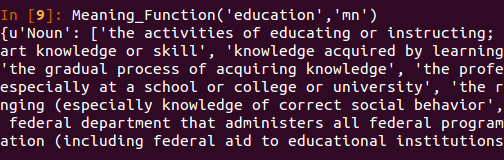
\includegraphics[width=0.75\linewidth]{dict.png}
	\end{figure}
	\begin{figure}
		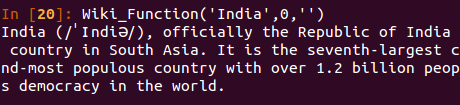
\includegraphics[width=0.75\linewidth]{wiki.png}
	\end{figure}

}

\frame{\frametitle{Outline of work to be done}
	\begin{itemize}
		\item Identifying underlined text\\
		\item Text to speech\\
	\end{itemize}
}

\end{document}
